\documentclass[aps,prd,superscriptaddress,floatfix]{revtex4}


\usepackage{graphicx}  
\usepackage{dcolumn}   
\usepackage{bm}        
\usepackage{amssymb}   



 

\begin{document}

\author {Matthew Herndon}

\address{University of Wisconsin, Madison, Wisconsin, USA}

\date{\today}


\title{  
\vspace{0.5cm}
Planar Strip Detector Geometry Description
}


\begin{abstract}
\vskip 0.5cm
\noindent
This document describes the geometry class used to describe a planer strip
detector immersed in a magnetic field used to measures charged particle helical trajectories three dimensions.  
\end{abstract}

\maketitle

\vspace{0.3cm}


\section{Introduction}
The detector consists of a ten layer strip detector immersed in a 1
Tesla magnetic field.  The sensors are planes in the x,z plane with
the normals vectors along the y axis, though an arbitrary orientation is supported.
The sensors are grouped in 5 pairs with each pair closely spaced in y.  One sensor of each pair
measures in the x  direction (X sensors) while the other sensor measures in either the z direction (Z sensors) 
or at a +,-10 degree angle small angle (small angle sensors SAS)relative to the x direction.  The SAS allow matching
between Hits in the X view and the Z view.  The sensors closest to the iteration region are smaller in x and z and
have finer segmentation.  The magnetic field is oriented in the z direction to give
bending in the x,y plane. 
\\

The interaction vertex is at located 0,0,0 and particles generally move in the positive y direction.  
\\

The sensors are described by:
\begin{itemize}
\item   unsigned int type, types 0: X, 1, SAS, 2, Z
\item  unsigned int nStrips
\item   double stripPitch, nStrips times stripPitch gives the size in the measurement direction measurementSize
\item   double intrinsicHitResolution
\item   double hitResolution
\item   double badHitResolution
\item  double threshold
\item  TVector3 center
\item  TVector3 normal
\item  TVector3 measurementDirection, the cross produce of the normal and the measurementDirection give the strip or perpendicular direction.
\item  double \_perpSize;
\end{itemize}

This detector could represent a set of rectangular planes used in a fix target experiment
or a single wedge in phi of the cylindrical collider experiment, where additional identical
wedges could populate the cylinder to complete the cylindrical
design.  Further the detector could represent silicon or other
tracking strip detectors, calorimeter strip chambers, or muon
chambers given appropriate size and resolutions.

\section{Units}
 The detector and magnetic field and calculation of trajectories and particle properties are set up such that the units are distance (m), Energy (GeV), magnetic field (Tesla).


\section{Detector layout and performance}
In the default configuration the X strip sensors are oriented perpendicular to the y axis in
the x-z plane in 20 cm intervals.  Strips in the X sensors run in the z
direction.  The two inner, lowest y,  sensors have strips spaced 50
and 100 micron intervals in x, while the 3 outer sensors have strips spaced in 200 micron
intervals in x.  Each sensor has 4096 strips symmetrically positioned
around x = 0.  The magnetic filed is oriented in the z direction such
that each sensor makes measurements of the x-y position allowing
the curvature or pT to be measured in the magnetic field.

In the default configuration the Z strip sensors are oriented perpendicular to the y axis in
the x-z plane in 20 cm intervals.  Strips in the Z sensors run in the x
direction.  The two inner, lowest y,  sensors have strips spaced 50
and 100 micron intervals in x. While the next outer sensor has strips spaced in 200 micron
intervals in x.  Each sensor has 2048 strips symmetrically positioned
around z = 0.  Each sensor makes measurements of the x-z position allowing
the z component of the momentum to be measured.

In the default configuration the SAS strip sensors are oriented perpendicular to the y axis in
the x-z plane in 20 cm intervals.  Strips in the SAS sensors run
+10 and -10 degree in angles from the x
direction.  The SAS sensors are at higher y than the Z sensors.  The  sensors have strips spaced 200 micron
intervals.  The sensors are placed 200 microns from the associated X sensor to allow measurement in X
and SAS to be used to find an intersections which determines the z coordinate and match the information from the X sensors with the 
information from the Z sensors .  Without partially rotated SAS sensors the X an Z views would be independent making it impossible to match X and Z
views.

Figure ~\ref{fig:detector} shows a view of the detector with one track and associated hits superimposed.

\begin{figure}[hbtp]
  \begin{center}
    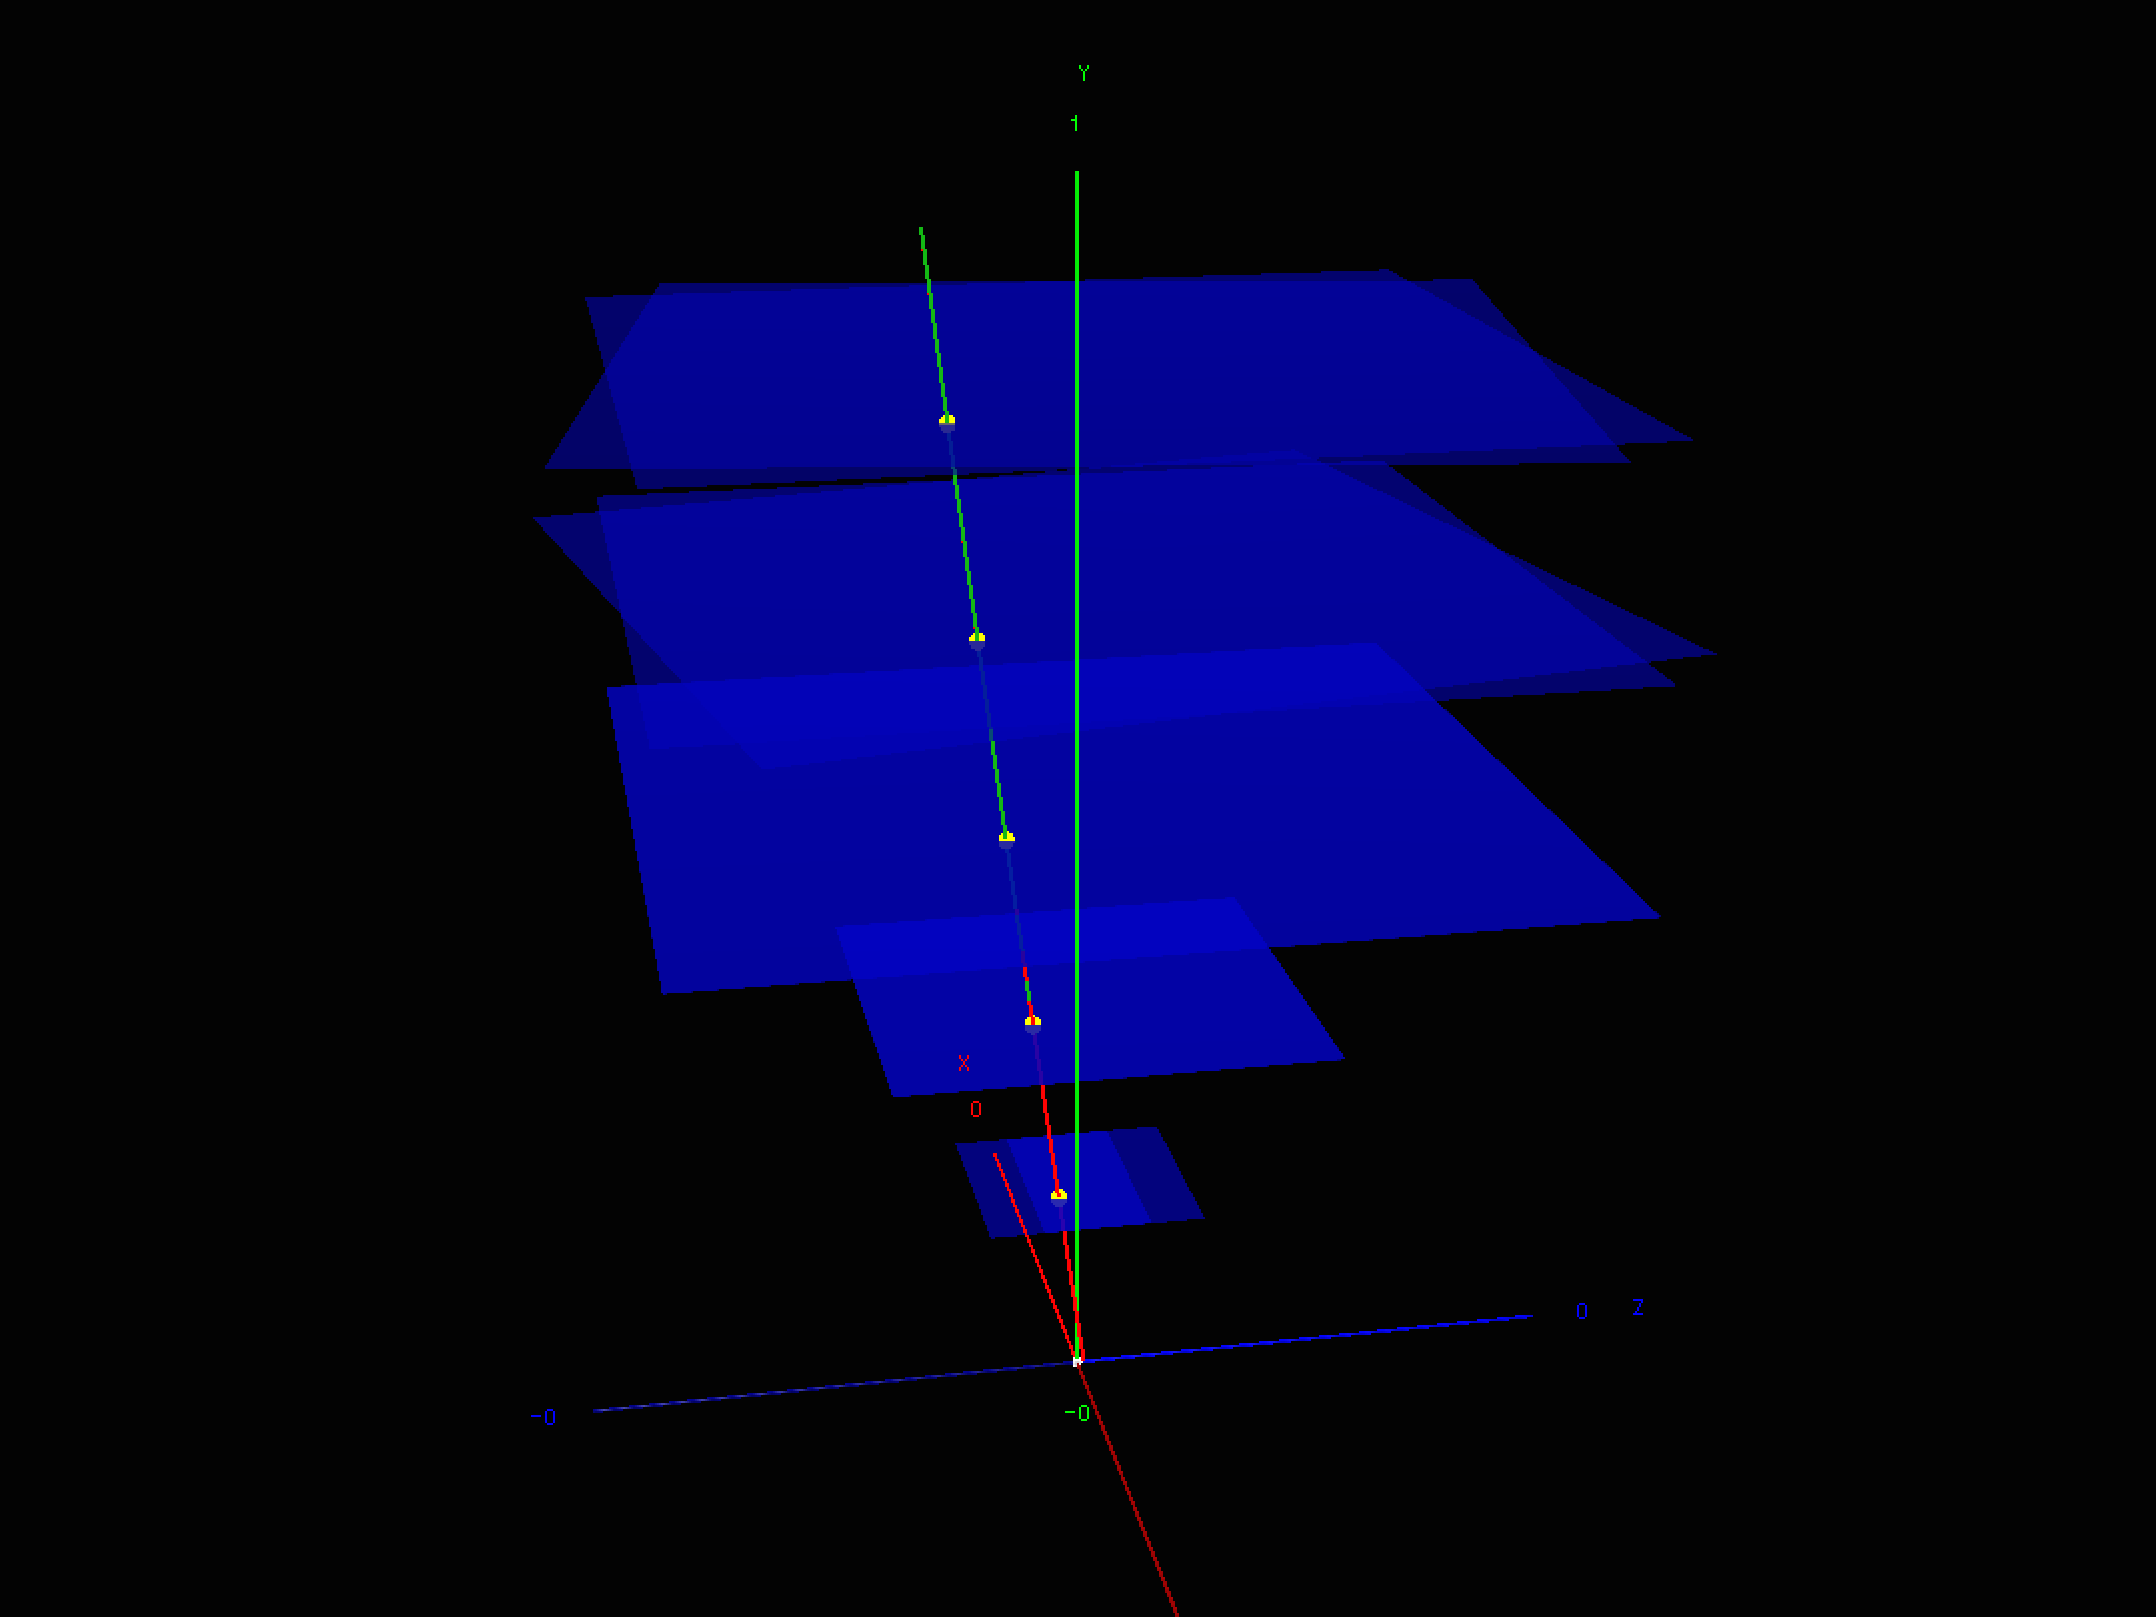
\includegraphics[width=17.0cm]{detector.png}
   \caption{Toy detector geometry with a track and associated hits superimposed}
    \label{fig:detector}
  \end{center}
\end{figure}


The sensors digitize approximately 64 ADC counts of charge per charged
particle hit and have a hit resolution given in microns which is due to
digitization and intrinsic resolution uncertainties.  Charge
deposition is taken as minimum ionizing and set to 32 ADC counts.  The combined resolution
due to intrinsic resolution and digitization uncertainty can be measured using the simulation by comparing true generated and reconstructed
hit positions.  In addition when only one strip is hit or when two hits from
different tracks overlap resolution can be degraded.  However, these cases can
be identified by the number of strips or the amount of charge in a hit and separate
resolutions for ``bad'' hits can be assigned.
\\

A subset of the sensor characteristics is given in table~\ref{tab:detectorTable}
\\

\begin{table}
\caption{\label{tab:detectorTable} Sensor properties.}
\begin{tabular}{|l|l|l|l|l|l|}
\hline 
Layer & type & Number Strips & Strip Pitch (um) & Y Pos (m) & Res (um)\\
\hline
0 & X & 2048 & 50	& 0.2 & 12	 \\
1 & X & 2048 & 100	& 0.4 & 25	 \\
2 & X & 2048 & 200	& 0.6 & 50	 \\
3 & X & 2048 & 200	& 0.8 & 50	 \\
4 & X & 2048 & 200	& 1.0 & 50	 \\
5 & Z & 2048 & 50	& 0.2002 & 12	 \\
6 & Z & 2048 & 100	& 0.4002 & 25	 \\
7 & Z & 2048 & 200	& 0.6002 & 50	 \\
8 & SAS & 2048 & 200	& 0.8002 & 50	 \\
9 & SAS & 2048 & 200	& 1.0002 & 50	 \\
\hline
\end{tabular}
\end{table}

In addition the primaryVertex is also described as a 0.01(m) resolution ``sensor'' in X and Z to allow
for performing a primaryVertex constraint to determine a track trajectory from 2X and one SAS
hit.  With the primary vertex and 2 hits a circle can be determined in the XY plane and the primary
vertex and one Z or SAS hit can be used to determine the trajectory in z.


Detector geometry class variables:
\begin{itemize}
\item int, \_nXSensors, \_nZSensors, \_nSASSensors 
\item int \_MIP: 
\item TVector3 \_bField: magnetic field strength, oriented along z-axis
\item \_curvatureC: allows conversion between pT and curvature using units of Tesla, meters, and GeV
\item \_sensors, vector of Sensors classes: describing the sensors
\end{itemize}

Detector geometry class functions:
\begin{itemize}
\item vector of Sensor type sensors(), get vector of all sensors
\item Sensor sensor(int layer) get one sensor, -2 and -1 are for the X and Z
  primary vertex information and layers 0 - N-1 for the N physical
  sensors
\item int nSensors() total sensor vector size
\item double curvatureCInField(TVector3 bField) curvature constant in arbitrary field
\item int nXSensors()
\item all other accessors are named according to their class variables
  as is nXSensors() is named for \_nXSensors
\end{itemize}




\end{document}
